\documentclass[border=2pt]{standalone}
\usepackage[dvipsnames,svgnames,x11names]{xcolor}
\usepackage{tikz}
\usetikzlibrary{arrows.meta,shapes.geometric}
\begin{document}
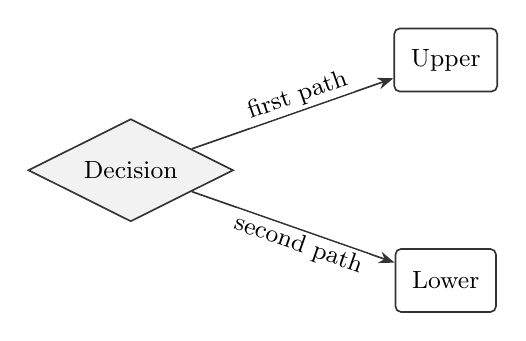
\begin{tikzpicture}[font=\small,>=Stealth]
\node[diamond,aspect=2,fill=black!5,draw=black!80,text=black,line width=0.6pt,minimum height=8mm,inner xsep=6pt,inner ysep=4pt,align=center] (choice) at (0,0) {Decision};
\node[rectangle,rounded corners=2pt,fill=white,draw=black!80,text=black,line width=0.6pt,minimum height=8mm,inner xsep=6pt,inner ysep=4pt,align=center] (upper) at (4,1.4) {Upper};
\node[rectangle,rounded corners=2pt,fill=white,draw=black!80,text=black,line width=0.6pt,minimum height=8mm,inner xsep=6pt,inner ysep=4pt,align=center] (lower) at (4,-1.4) {Lower};
\draw[->,draw=black!80,line width=0.6pt] (choice) -- node[pos=0.55,above,sloped,fill=white,inner sep=1.2pt] {first path} (upper);
\draw[->,draw=black!80,line width=0.6pt] (choice) -- node[pos=0.55,below,sloped,fill=white,inner sep=1.2pt] {second path} (lower);
\end{tikzpicture}
\end{document}
